% ============================================================================
% Geophysical Journal International (GJI) manuscript
% Requires the GJI LaTeX class + bib style (gji.cls, gji.bst), available from the
% GJI author guidelines / OUP LaTeX template. If gji.cls is unavailable, replace
%   \documentclass[extra,mreferee]{gji}
% with
%   \documentclass[12pt]{article}\usepackage{natbib,graphicx,amsmath,amssymb}
% and remove the GJI-only commands (\summary, \keywords, \pubyear, \volume, ...).
% Compile: pdflatex -> bibtex -> pdflatex -> pdflatex
% ============================================================================
\documentclass[extra,mreferee]{gji}

\usepackage{amsmath}
\usepackage{amssymb}
\usepackage{graphicx}
\graphicspath{{../figures/moho/}}

\title[The Moho of Indonesia from satellite gravity]
      {The Moho of Indonesia from satellite gravity: a fast spherical
       Bott--Tikhonov inversion validated against seismic estimates}

\author[M. Zuhdi, Sudarmaji \& W. Suryanto]{%
  Muhammad Zuhdi,$^{1}$ Sudarmaji$^{1}$ and Wiwit Suryanto$^{1}$\thanks{%
  Corresponding author: Wiwit Suryanto (\texttt{[email]})}\\
  $^{1}$Geophysics Laboratory, Universitas Gadjah Mada, Sekip Utara PO BOX BLS 21,
  Yogyakarta 55281, Indonesia}

\date{Received --- ; in original form ---}
\pubyear{2026}

\begin{document}
\label{firstpage}
\maketitle

\begin{summary}
The depth of the Mohorovi\v{c}i\'{c} discontinuity (Moho) is a first-order
constraint on crustal structure, yet across the Indonesian archipelago it is
known only unevenly, mostly from sparse seismic stations. We estimate the Moho of
Indonesia ($94^{\circ}$--$141^{\circ}$E, $15^{\circ}$S--$6^{\circ}$N) from
satellite gravity by adapting the fast, regularized, spherical inversion of
\citet{uieda2017}: the anomalous Moho is discretized into tesseroids, forward
modelled on a spherical Earth, and inverted with Bott's method stabilized by
first-order Tikhonov regularization. Gravity disturbances are derived from the
satellite-only global model {GOCO06s} and corrected for topography and bathymetry
with tesseroids. The three hyperparameters --- regularization weight $\mu$,
density contrast $\Delta\rho$ and reference depth $z_{\mathrm{ref}}$ --- are
estimated by hold-out cross-validation and by validation against a compilation of
105 receiver-function Moho depths. The preferred model
($\mu=10^{-10}$, $z_{\mathrm{ref}}=35$~km, $\Delta\rho=500$~kg\,m$^{-3}$) fits the
seismic Moho with a mean difference of $+1.2$~km and a standard deviation of
$5.8$~km, comparable to the original South American application ($1.2$, $6.8$~km).
An independent comparison with the seismic {AusMoho} model along the northern
Australian margin shows near-zero bias ($-0.1$~km) and strong correlation
($r=0.86$). The gravity Moho is thick ($35$--$45$~km) beneath the Sunda, Sulawesi
and Banda arcs and the Papuan highlands, and thin ($10$--$20$~km) beneath the
marginal and oceanic basins, and co-varies with the trenches, active faults and
volcanic arc. We show that the seismic misfit decreases monotonically with
$\Delta\rho$ (a density--depth trade-off), so $\Delta\rho$ is best read as an
effective contrast constrained by independent data rather than a tightly
determined physical quantity.
\end{summary}

\begin{keywords}
Inverse theory -- Satellite gravity -- Gravity anomalies and Earth structure --
Crustal structure -- Indonesia.
\end{keywords}

% ============================================================================
\section{Introduction}
% ============================================================================
The Mohorovi\v{c}i\'{c} discontinuity separates crust from mantle and is a primary
target in studies of lithospheric structure, isostasy and geodynamics. In
tectonically complex regions such as Indonesia --- where the Indo-Australian,
Sunda, Philippine Sea and Pacific plates interact through subduction, collision
and back-arc spreading --- Moho depth varies strongly over short distances.
Seismic methods (receiver functions, refraction, ambient-noise tomography) give
the most direct estimates but are limited to the vicinity of stations, which in
Indonesia are concentrated on land and along the volcanic arc.

Gravity provides continuous, homogeneous coverage and is well suited to mapping
the crust--mantle interface at regional scale, especially offshore where satellite
missions give near-uniform data. Estimating an interface such as the Moho from
gravity is a nonlinear, ill-posed inverse problem. \citet{uieda2017} introduced a
computationally efficient solution in \emph{spherical} coordinates that combines
(i) Bott's \citep{bott1960} iterative method, which avoids forming a dense
Jacobian; (ii) tesseroid (spherical-prism) forward modelling \citep{uieda2016},
which respects Earth curvature at continental-to-global scale; and (iii)
first-order Tikhonov regularization for stability, and applied it to the South
American Moho.

Here we transfer that methodology, unchanged in principle, to the whole of
Indonesia. Our objectives are to (1) produce a reproducible, public-data gravity
Moho model of the Indonesian region; (2) calibrate and validate it against an
independent compilation of seismic Moho depths, and cross-check it against the
seismic {AusMoho} model \citep{kennett2011} at the Australian margin; and (3)
examine how the gravity Moho relates to the region's tectonic framework. We keep
the method identical to \citet{uieda2017} so that differences reflect the data and
tectonic setting rather than the algorithm.

% ============================================================================
\section{Data}
% ============================================================================
\textbf{Satellite gravity.} We use the satellite-only global gravity model
{GOCO06s} \citep{kvas2021}, the successor of the {GOCO5s} model used by
\citet{uieda2017}, synthesised to spherical-harmonic degree/order 300 on a regular
grid at a constant height of 4~km above the {WGS84} ellipsoid. For a
higher-resolution variant we also use the altimetry-derived free-air gravity
anomaly \citep{sandwell2014} as a proxy for the disturbance.

\textbf{Topography/bathymetry.} Earth relief is taken from {SRTM15+}
\citep{tozer2019}, resampled to the model grid.

\textbf{Seismic Moho.} An independent compilation of 105 receiver-function Moho
depths at seismic stations spanning $96^{\circ}$--$141^{\circ}$E,
$10^{\circ}$S--$5^{\circ}$N (depths 20--40~km) is used to calibrate
$z_{\mathrm{ref}}$ and $\Delta\rho$ and to assess the model
\textbf{[cite the compilation source and confirm the depth datum]}.

\textbf{Auxiliary data.} Active faults, fold axes and the Sunda--Banda trench are
from \textbf{[cite the active-fault dataset]}; Holocene volcanoes are from the
Smithsonian Global Volcanism Program \citep{gvp2013}; sedimentary basins and
thickness from {CRUST1.0} \citep{laske2013} and the Indonesian basin maps of
\citet{darman2020} and \citet{esdm2022}; and the northern-Australia cross-check
from the {AusMoho} grid \citep{kennett2011}.

% ============================================================================
\section{Methods}
% ============================================================================
\subsection{Gravity disturbance}
The gravity disturbance at an observation point $P$ is
\begin{equation}
\delta(P) = g(P) - \gamma(P),
\label{eq:disturbance}
\end{equation}
where $g(P)$ is the {GOCO06s} gravity synthesised at constant height and
$\gamma(P)$ the closed-form {WGS84} normal gravity. The disturbance contains only
the effects of masses anomalous with respect to the reference ellipsoid.

\subsection{Forward modelling with tesseroids}
All mass effects are computed on a spherical Earth using tesseroids, which honour
Earth curvature at regional scale. A tesseroid bounded by longitudes
$[\lambda_1,\lambda_2]$, latitudes $[\phi_1,\phi_2]$ and radii $[r_1,r_2]$, of
constant density $\rho$, produces at $P=(r_P,\phi_P,\lambda_P)$ the potential
\begin{equation}
V(P) = G\rho \int_{\lambda_1}^{\lambda_2}\!\!\int_{\phi_1}^{\phi_2}\!\!\int_{r_1}^{r_2}
       \frac{r^2\cos\phi}{\ell}\; dr\,d\phi\,d\lambda,
\label{eq:potential}
\end{equation}
where $G$ is the gravitational constant and
$\ell=(r_P^2+r^2-2r_Pr\cos\psi)^{1/2}$, with
$\cos\psi=\sin\phi_P\sin\phi+\cos\phi_P\cos\phi\cos(\lambda-\lambda_P)$. The
modelled datum is the radial component of the attraction,
\begin{equation}
g_z(P) = -\frac{\partial V}{\partial r_P}
       = G\rho \int_{\lambda_1}^{\lambda_2}\!\!\int_{\phi_1}^{\phi_2}\!\!\int_{r_1}^{r_2}
         \frac{(r_P-r\cos\psi)\,r^2\cos\phi}{\ell^{3}}\; dr\,d\phi\,d\lambda,
\label{eq:gz}
\end{equation}
which has no analytical solution and is evaluated by Gauss--Legendre Quadrature
with the adaptive discretization of \citet{uieda2016}.

The anomalous Moho is parameterised as $M$ juxtaposed tesseroids, one per grid
cell, each spanning the radial gap between the reference Moho at radius
$R-z_{\mathrm{ref}}$ and the true Moho at $R-z_k$; the unknowns are the depths
$\mathbf{p}=(z_1,\dots,z_M)^{T}$. A cell deeper than the reference
($z_k>z_{\mathrm{ref}}$) is assigned contrast $-\Delta\rho$ (a mass deficit) and a
shallower cell $+\Delta\rho$ \citep{uieda2017}. The predicted gravity at the $N$
observation points is the nonlinear forward map
\begin{equation}
d_i(\mathbf{p}) = f_i(\mathbf{p}) = \sum_{k=1}^{M} g_z^{(k)}(P_i;\,z_k),
\qquad i=1,\dots,N.
\label{eq:forward}
\end{equation}

\subsection{Data corrections}
The topographic/oceanic effect $g_{\text{topo}}$ (tesseroids; land density
$2670$~kg\,m$^{-3}$, ocean contrast $\approx-1640$~kg\,m$^{-3}$) is removed to give
the Bouguer disturbance,
\begin{equation}
\delta_{bg}(P) = \delta(P) - g_{\text{topo}}(P).
\label{eq:bouguer}
\end{equation}
Optionally the {CRUST1.0} sediment effect $g_{\text{sed}}$ is removed, giving the
sediment-free Bouguer disturbance
$\delta_{sf}=\delta_{bg}-g_{\text{sed}}$, the inversion input $\mathbf{d}^{o}$.
The full reduction chain is shown in Fig.~\ref{fig:chain}.

\subsection{Inverse problem}
We minimise the data-misfit functional
\begin{equation}
\phi(\mathbf{p}) = [\mathbf{d}^{o}-\mathbf{d}(\mathbf{p})]^{T}
                   [\mathbf{d}^{o}-\mathbf{d}(\mathbf{p})].
\label{eq:misfit}
\end{equation}
Because \eqref{eq:forward} is nonlinear and the problem is ill-posed, we add
first-order Tikhonov (smoothness) regularization
$\theta(\mathbf{p})=\mathbf{p}^{T}\mathbf{R}^{T}\mathbf{R}\,\mathbf{p}$, where
$\mathbf{R}$ is the first-difference operator between adjacent depths, and
minimise the goal function
\begin{equation}
\Gamma(\mathbf{p}) = \phi(\mathbf{p}) + \mu\,\theta(\mathbf{p}).
\label{eq:goal}
\end{equation}
$\Gamma$ is minimised by Gauss--Newton: at iteration $k$ the perturbation
$\Delta\mathbf{p}^{k}$ solves
\begin{equation}
\big(\mathbf{A}^{k\,T}\mathbf{A}^{k} + \mu\,\mathbf{R}^{T}\mathbf{R}\big)
   \Delta\mathbf{p}^{k} =
   \mathbf{A}^{k\,T}[\mathbf{d}^{o}-\mathbf{d}(\mathbf{p}^{k})]
   - \mu\,\mathbf{R}^{T}\mathbf{R}\,\mathbf{p}^{k},
\label{eq:gaussnewton}
\end{equation}
where $A_{ij}=\partial f_i/\partial z_j$. Following \citet{bott1960}, recast as a
Gauss--Newton special case by \citet{silva2014}, the dense Jacobian is replaced by
the diagonal Bouguer-plate approximation
\begin{equation}
\mathbf{A} = -2\pi G\,\Delta\rho\;\mathbf{I},
\label{eq:jacobian}
\end{equation}
the minus sign expressing that a deeper Moho lowers the gravity. With
\eqref{eq:jacobian} the term $\mathbf{A}^{T}\mathbf{A}=(2\pi G\Delta\rho)^{2}\mathbf{I}$
is diagonal and constant, so \eqref{eq:gaussnewton} is a sparse, symmetric
positive-definite system, factorised once and back-substituted each iteration. The
model is updated,
\begin{equation}
\mathbf{p}^{k+1} = \mathbf{p}^{k} + \Delta\mathbf{p}^{k},
\label{eq:update}
\end{equation}
with each $z_k$ clipped to $3$--$70$~km, and iterated until the change in RMS
misfit falls below the noise level. For $\mu=0$, \eqref{eq:gaussnewton}--%
\eqref{eq:update} reduce to the classical Bott update
$\Delta z_j = [d^{o}_j - d_j(\mathbf{p}^{k})]/(2\pi G\Delta\rho)$.

\subsection{Hyperparameters and resolution}
The hyperparameters $\mu$, $\Delta\rho$ and $z_{\mathrm{ref}}$ are estimated in two
steps \citep{uieda2017}: $\mu$ by hold-out cross-validation on the gravity data,
then $(z_{\mathrm{ref}},\Delta\rho)$ by validation against the seismic Moho
(Fig.~\ref{fig:hyper}). We invert on $0.5^{\circ}$ and $0.25^{\circ}$ grids with
both the {GOCO06s} satellite and altimetry gravity to separate grid resolution
from data resolution.

% ============================================================================
\section{Results}
% ============================================================================
\textbf{Calibrated hyperparameters.} Cross-validation selects $\mu=10^{-10}$
(essentially unregularized). The $(z_{\mathrm{ref}},\Delta\rho)$ validation
surface (Fig.~\ref{fig:hyper}) has a broad, flat minimum, and the seismic misfit
\emph{decreases monotonically with increasing $\Delta\rho$}: the raw argmin runs
away to unphysical contrasts ($>600$~kg\,m$^{-3}$). This reflects the
non-uniqueness of gravity inversion --- $\Delta\rho$ trades off against
$z_{\mathrm{ref}}$ and Moho amplitude and absorbs unmodelled effects. We therefore
adopt a physically reasonable $\Delta\rho=500$~kg\,m$^{-3}$ (cf. $400$ in
\citealt{uieda2017}) with $z_{\mathrm{ref}}=35$~km, a choice independently
supported by the {AusMoho} comparison (Section~5). $\Delta\rho$ is thus an
\emph{effective} contrast, not a tightly determined physical quantity.

\textbf{Moho model and validation.} The preferred model yields Moho depths of
$\sim7$--$59$~km (Fig.~\ref{fig:moho}), thick beneath the arcs and continental
blocks and thin beneath the oceanic basins. It differs from the 105 seismic depths
by a mean of $+1.2$~km and a standard deviation of $5.8$~km
(Fig.~\ref{fig:validation}), comparable to the South American result.

\textbf{Resolution.} Refining the grid to $0.25^{\circ}$ with {GOCO06s} does not
improve the seismic fit because the satellite signal ($\approx0.5^{\circ}$) does
not support finer structure; substituting the altimetry gravity recovers a
near-zero bias and a more detailed map (Table~\ref{tab:res}).

\begin{table}
\caption{Difference between estimated and seismic Moho ($N=105$) by gravity source
and grid.}
\label{tab:res}
\begin{tabular}{llcc}
\hline
Gravity source & Grid & Mean (km) & Std (km)\\
\hline
{GOCO06s} (satellite) & $0.5^{\circ}$ & $+1.1$ & \textbf{5.8}\\
Altimetry & $0.5^{\circ}$ & $+1.4$ & 6.0\\
{GOCO06s} (satellite) & $0.25^{\circ}$ & $+3.2$ & 8.0\\
Altimetry & $0.25^{\circ}$ & $+0.9$ & 6.9\\
\hline
\end{tabular}
\end{table}

% ============================================================================
\section{Discussion}
% ============================================================================
\textbf{Tectonic correlation.} The gravity Moho is spatially organized by the
region's tectonics (Figs~\ref{fig:west}--\ref{fig:east}): thick crust follows the
volcanic arc and the collision zones of Sulawesi, the Banda arc and Papua, while
thin crust marks the oceanic marginal basins. Holocene volcanoes lie along the
thick-crust arc; the largest gravity--seismic misfits occur where density
anomalies unrelated to the Moho --- the subducting Sunda--Banda slabs and
volcanic/collisional bodies --- are not modelled, as in \citet{uieda2017}.

\textbf{Cross-validation with {AusMoho}.} Where our domain overlies the Australian
continental margin ($\sim132^{\circ}$--$140^{\circ}$E, $10^{\circ}$--$11^{\circ}$S),
our gravity Moho ($\sim33$--$37$~km) agrees with {AusMoho} \citep{kennett2011};
over the northern Australian mainland ($15^{\circ}$--$11.5^{\circ}$S, $N=369$
cells) the mean difference is $-0.1$~km, standard deviation $4.8$~km and
correlation $r=0.86$ --- encouraging agreement between two independent methods.
The main difference is thicker crust (39--50~km) at the Timor--Banda collision
front, consistent with collisional thickening.

\textbf{Limitations.} (1) Validation is land-biased and cannot constrain the
offshore Moho. (2) Resolution is limited by the satellite gravity, not the grid.
(3) The sediment correction had little benefit: {CRUST1.0} did not improve the
fit, and a correction built from station receiver-function sediment thicknesses
\citep{bahri2023} over-corrected --- the western Moho, already in near-zero-bias
agreement without any sediment correction, was pushed $\sim2$~km too shallow.
Because those thicknesses are thin ($\sim2$~km) and point-sampled, they miss the
basin depocenters the correction requires; a basin-scale sediment/depth-to-basement
map \citep{hardy1997,darman2020,esdm2022} would be needed. This indicates that
sediments are a minor effect at the validation points and are not the cause of the
$\Delta\rho$ trade-off. (4) The reference height and single density contrast are
simplifications inherited from the method.

% ============================================================================
\section{Conclusions}
% ============================================================================
We produced a reproducible, public-data gravity Moho model for the whole
Indonesian region using the fast spherical Bott--Tikhonov tesseroid inversion of
\citet{uieda2017}. Calibrated against 105 seismic Moho depths and cross-checked
against the independent {AusMoho} model, the model reproduces first-order
crustal-thickness variations and fits the seismic data to $5.8$~km. Estimated Moho
depth correlates with trenches, active faults and the volcanic arc, and the
largest gravity--seismic residuals coincide with subduction and collision fronts.
Resolution is limited by the satellite gravity rather than the model grid, and the
density contrast is best read as an effective parameter constrained by independent
data.

\section*{Data and code availability}
All code is openly available at
\texttt{https://github.com/maswiet/fbt-gravity-seismicity}. Input data are public:
{GOCO06s}, {SRTM15+}/altimetry via GMT, {CRUST1.0}, and the Smithsonian GVP volcano
list. The seismic-Moho compilation, the active-fault dataset and the {AusMoho} grid
are third-party.

\section*{Acknowledgments}
\textbf{[Add funding and data providers.]}

\bibliographystyle{gji}
\bibliography{refs}

% ============================================================================
% Figures
% ============================================================================
\begin{figure*}
\centering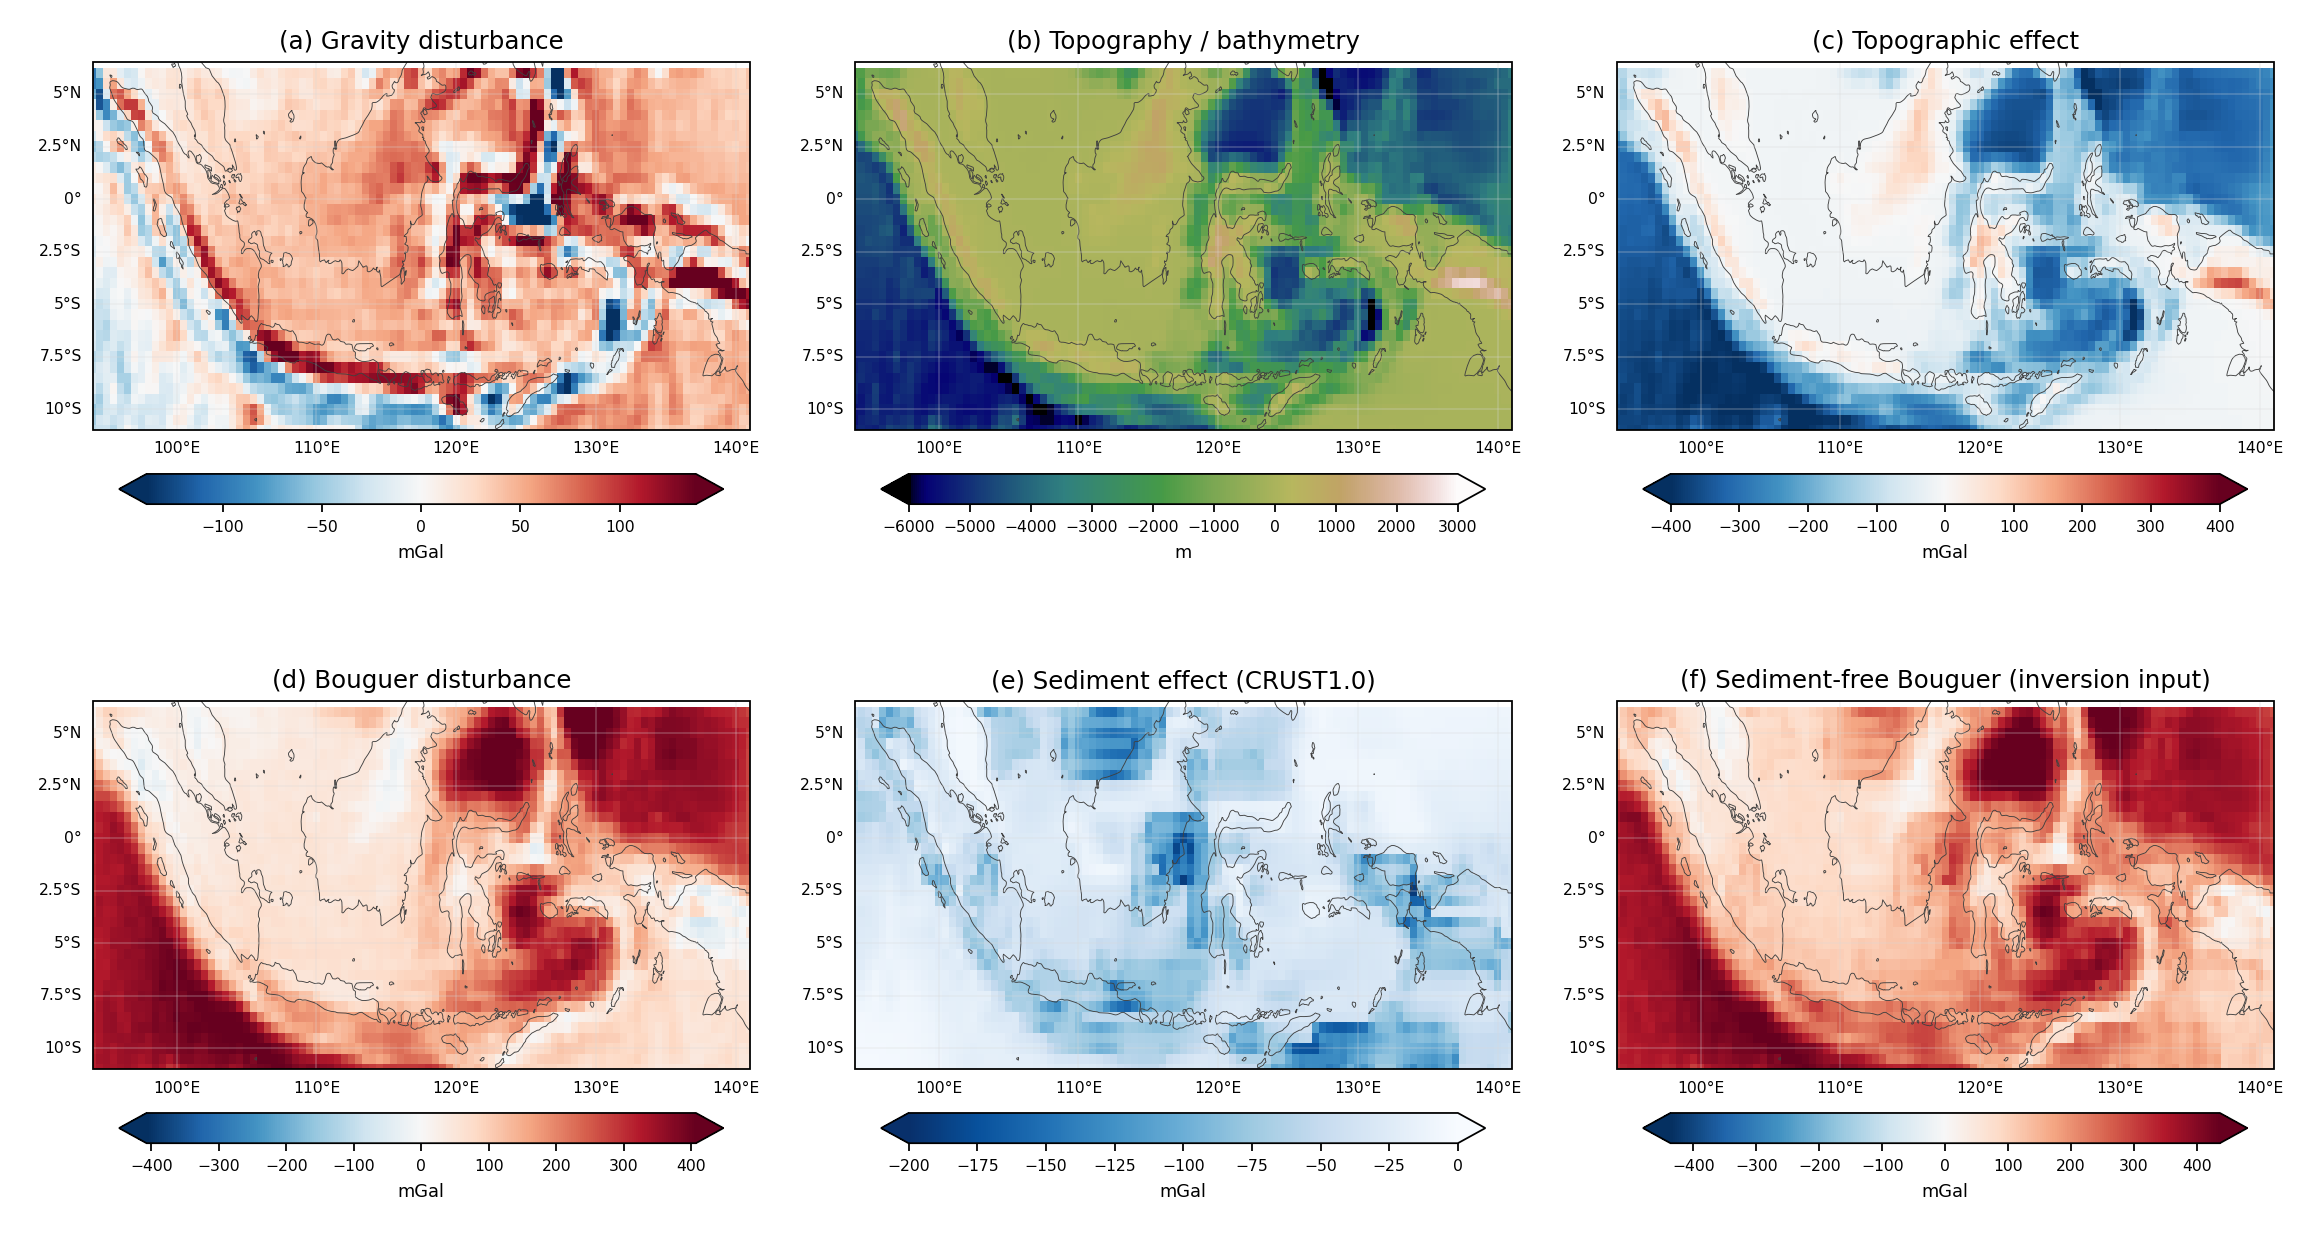
\includegraphics[width=\textwidth]{processing_chain.png}
\caption{Gravity data-reduction chain: (a) gravity disturbance, (b)
topography/bathymetry, (c) topographic effect, (d) Bouguer disturbance, (e)
{CRUST1.0} sediment effect, (f) sediment-free Bouguer disturbance (inversion
input).}
\label{fig:chain}
\end{figure*}

\begin{figure}
\centering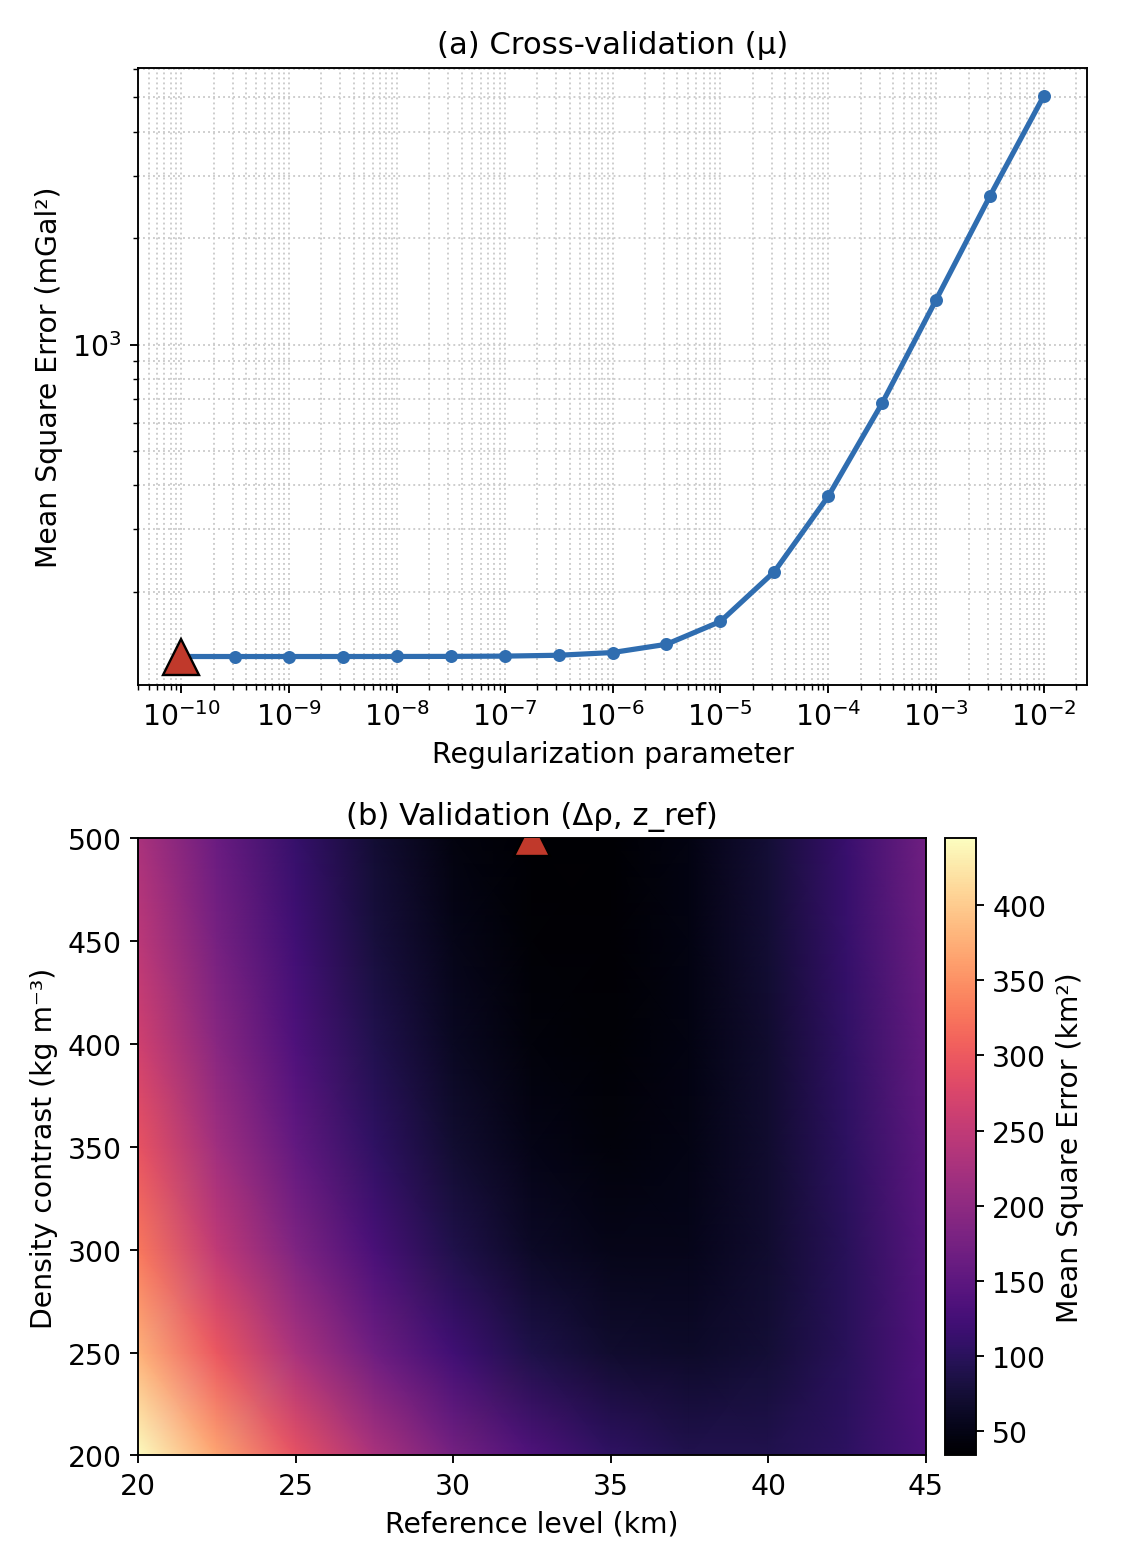
\includegraphics[width=\columnwidth]{hyperparameters.png}
\caption{Hyperparameter diagnostics. (a) $\mu$ hold-out cross-validation.
(b) $(z_{\mathrm{ref}},\Delta\rho)$ validation-MSE surface; the triangle marks the
adopted $z_{\mathrm{ref}}=35$~km, $\Delta\rho=500$~kg\,m$^{-3}$. The minimum is
broad and the misfit decreases monotonically with $\Delta\rho$.}
\label{fig:hyper}
\end{figure}

\begin{figure*}
\centering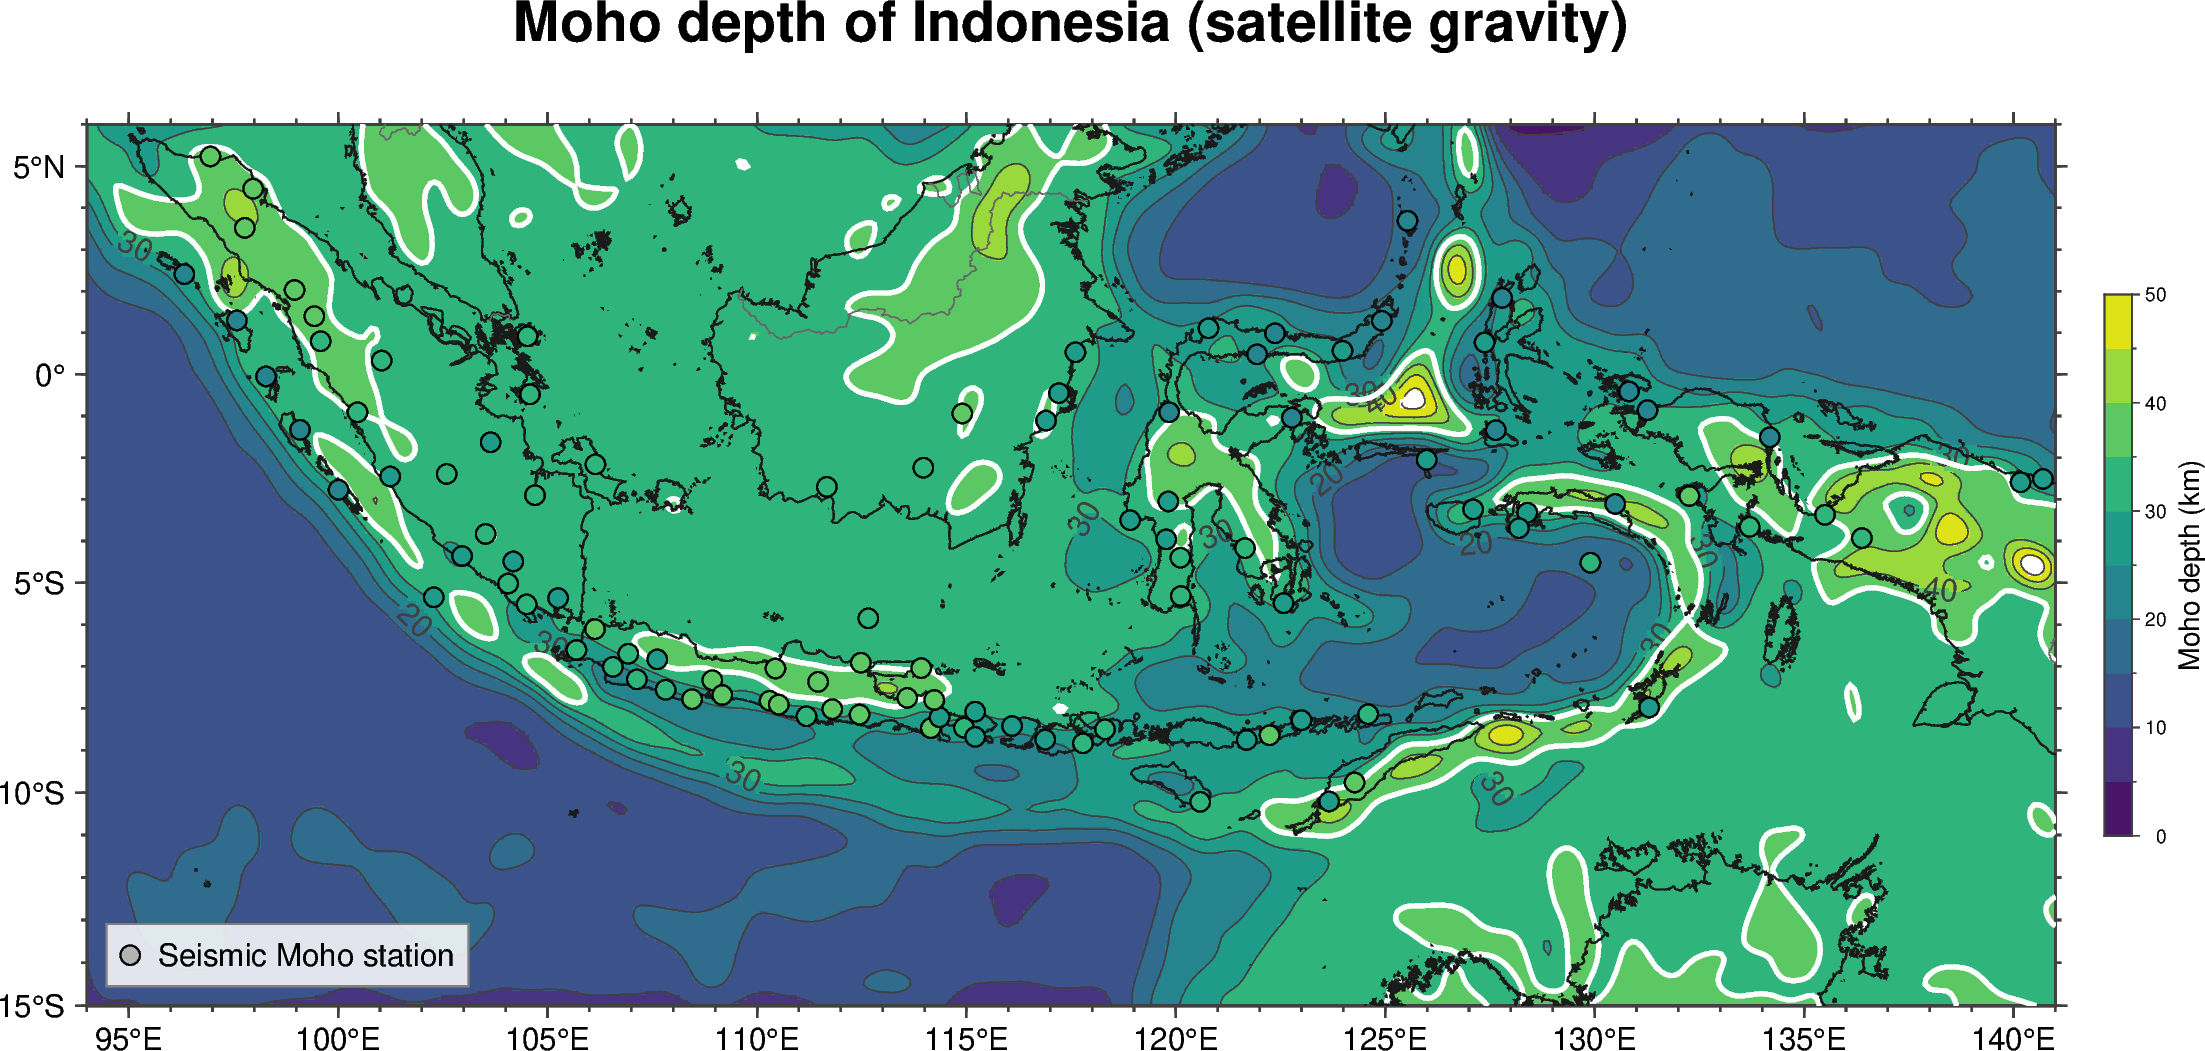
\includegraphics[width=\textwidth]{moho_full_clean.png}
\caption{Estimated Moho depth of Indonesia, with seismic Moho stations and depth
contours (35-km contour in white).}
\label{fig:moho}
\end{figure*}

\begin{figure}
\centering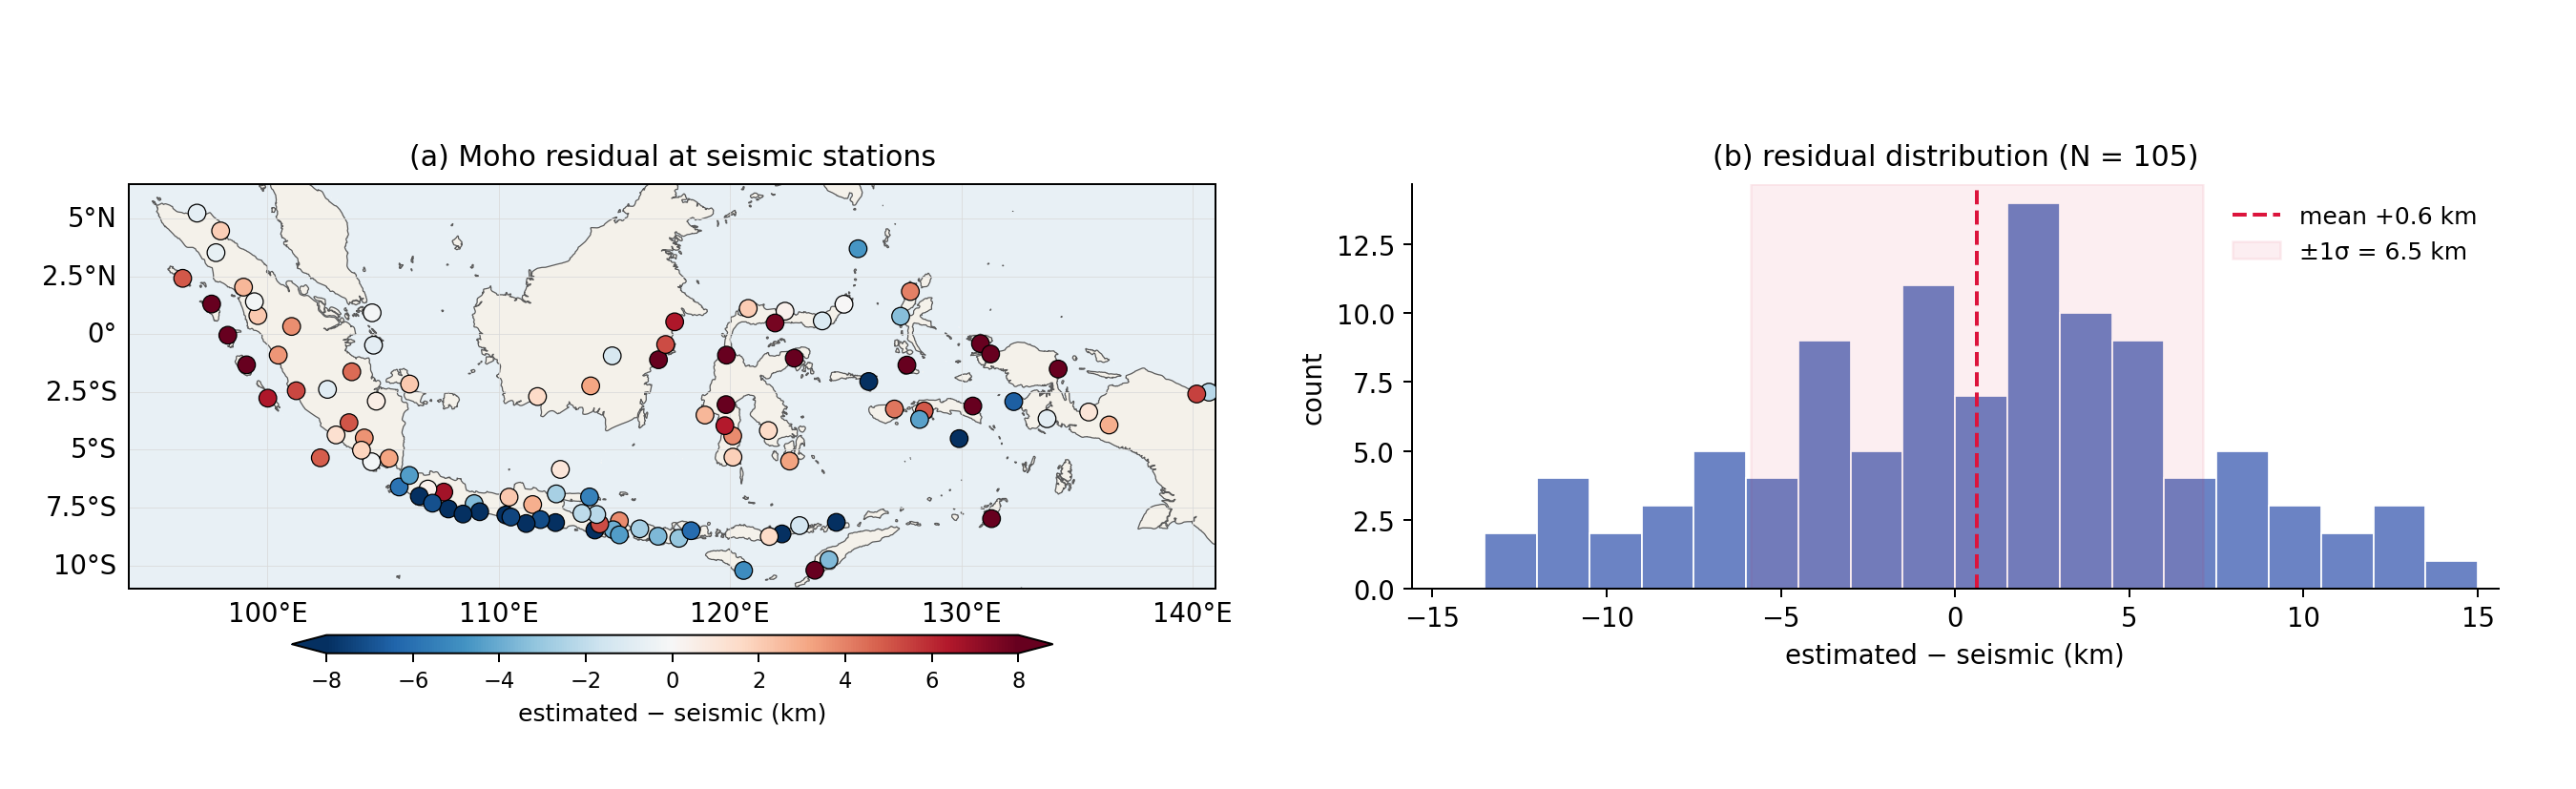
\includegraphics[width=\columnwidth]{validation_seismic.png}
\caption{Moho residual (estimated $-$ seismic) at the 105 stations: (a) map,
(b) histogram (mean $+1.2$, std $5.8$~km).}
\label{fig:validation}
\end{figure}

\begin{figure*}
\centering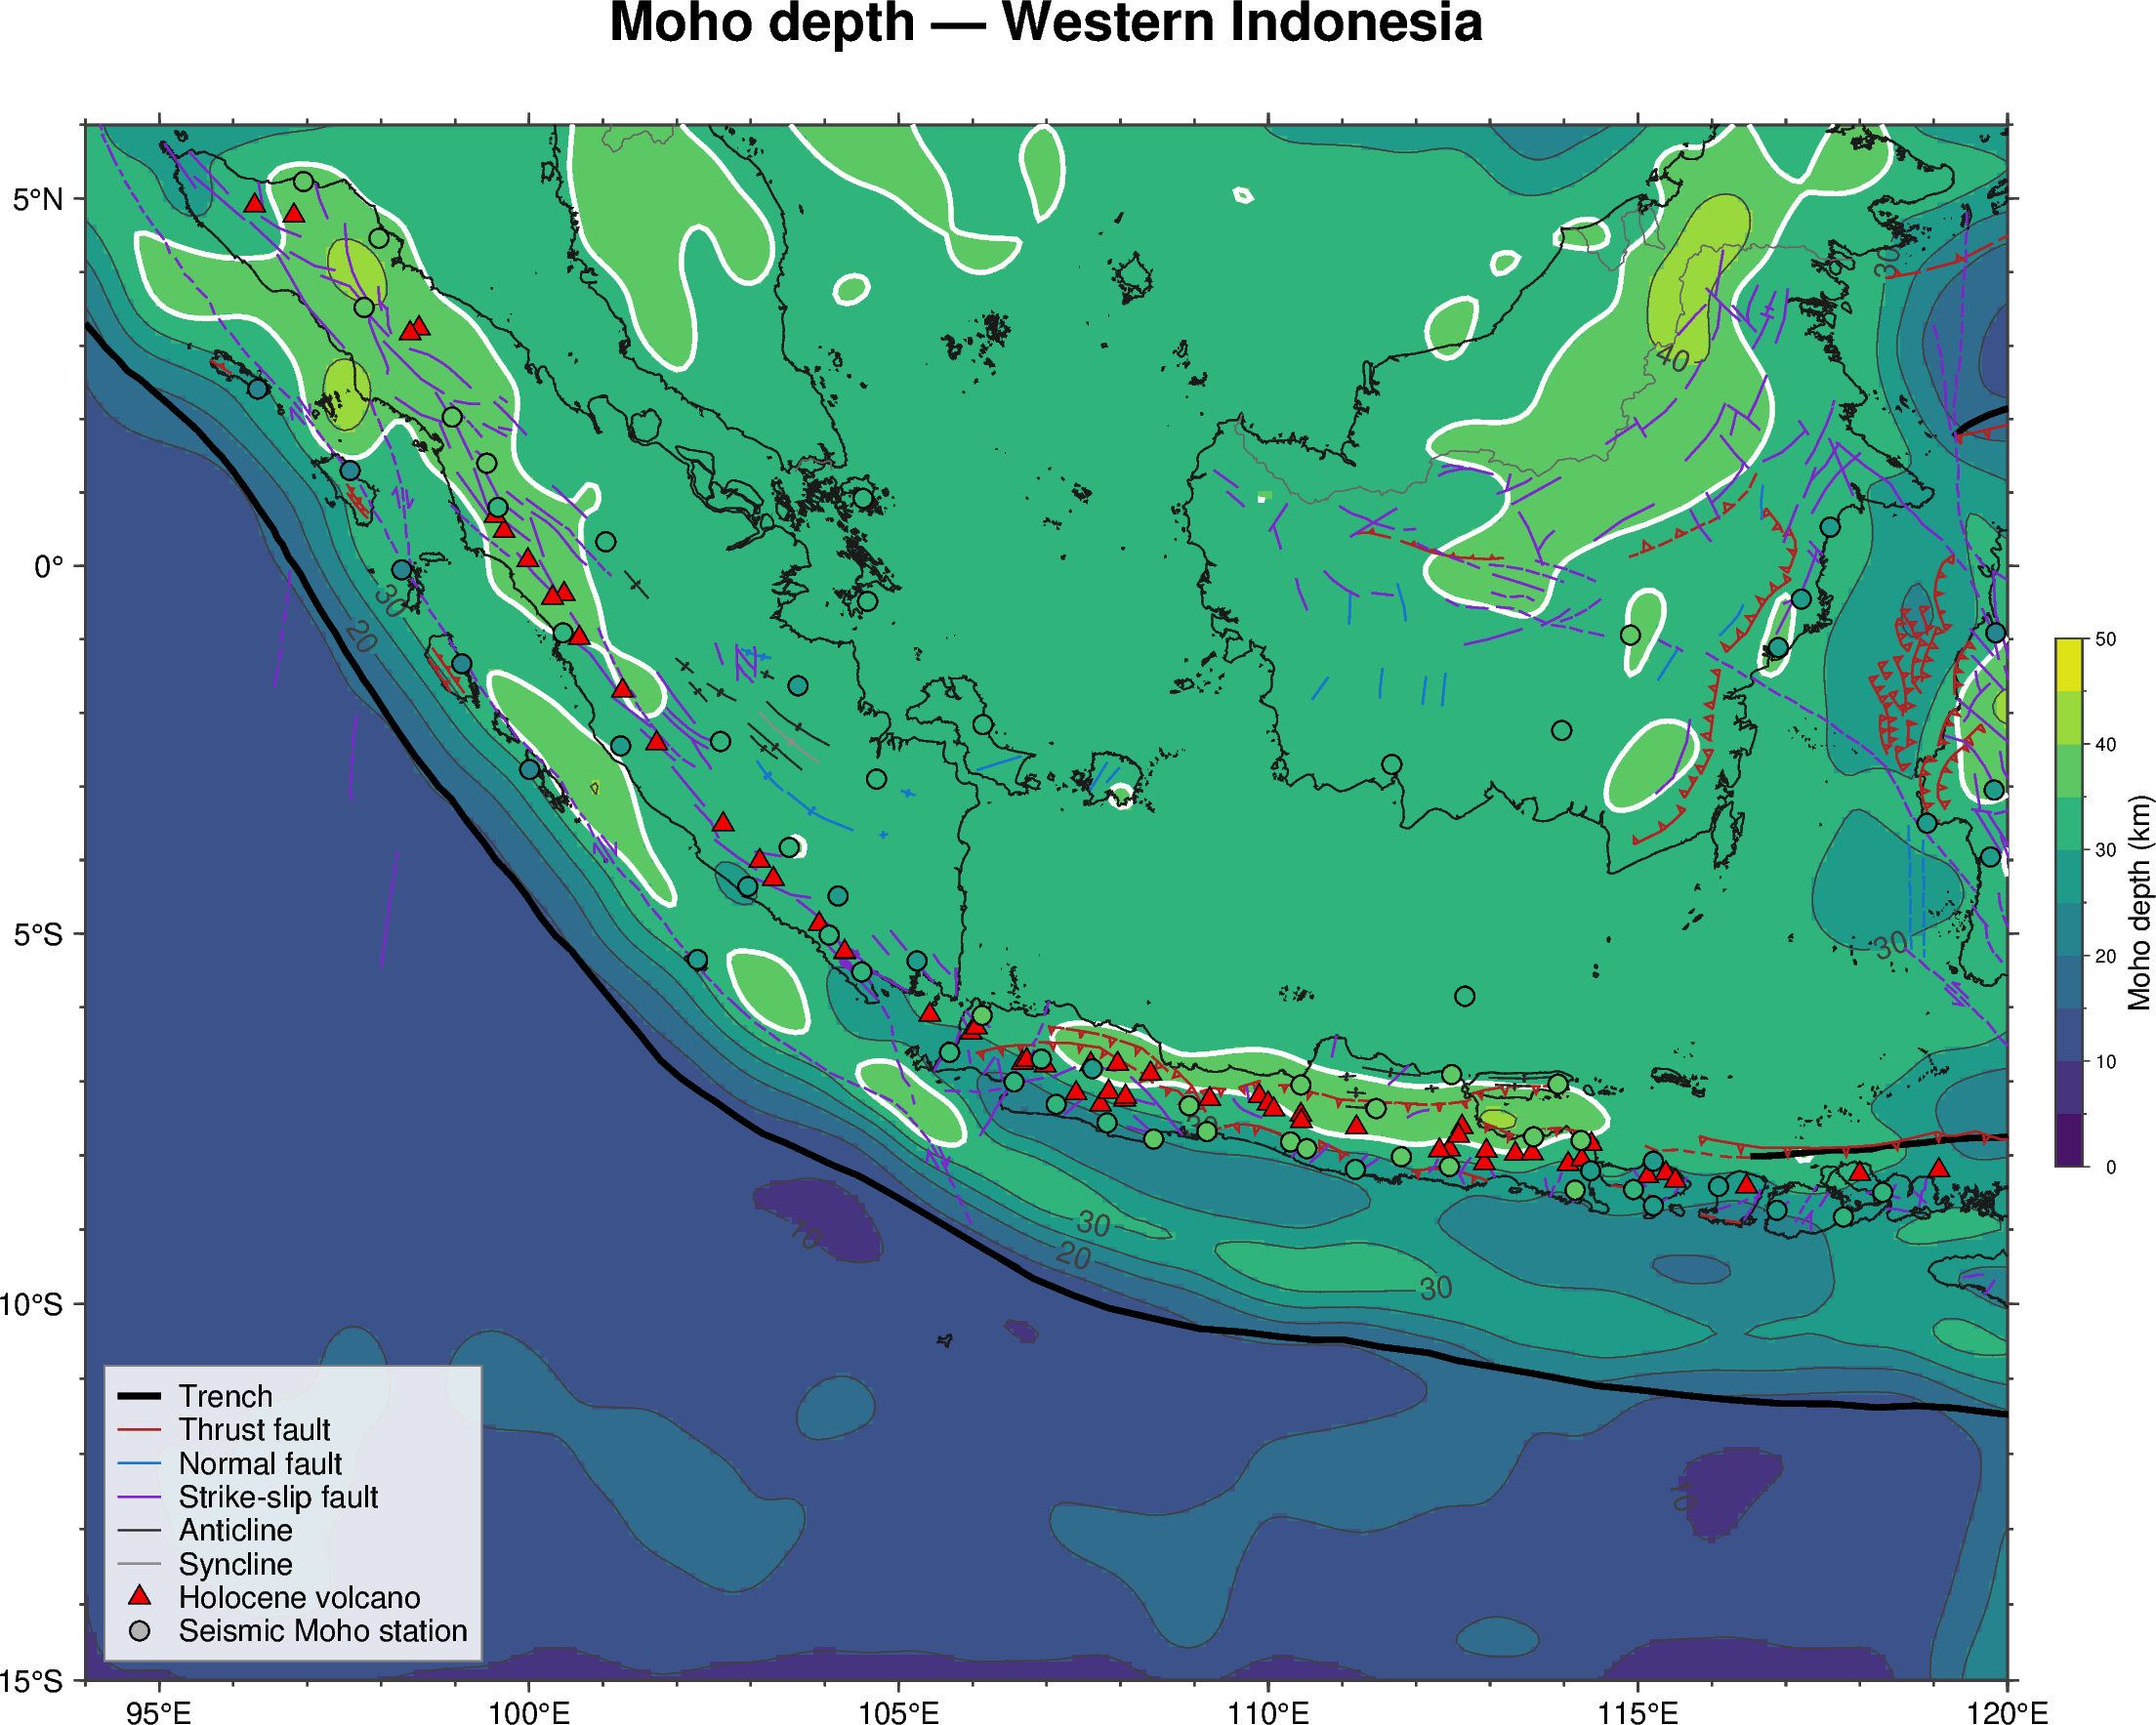
\includegraphics[width=\textwidth]{moho_west.png}
\caption{Western Indonesia: Moho depth with trench, active faults, fold axes and
Holocene volcanoes.}
\label{fig:west}
\end{figure*}

\begin{figure*}
\centering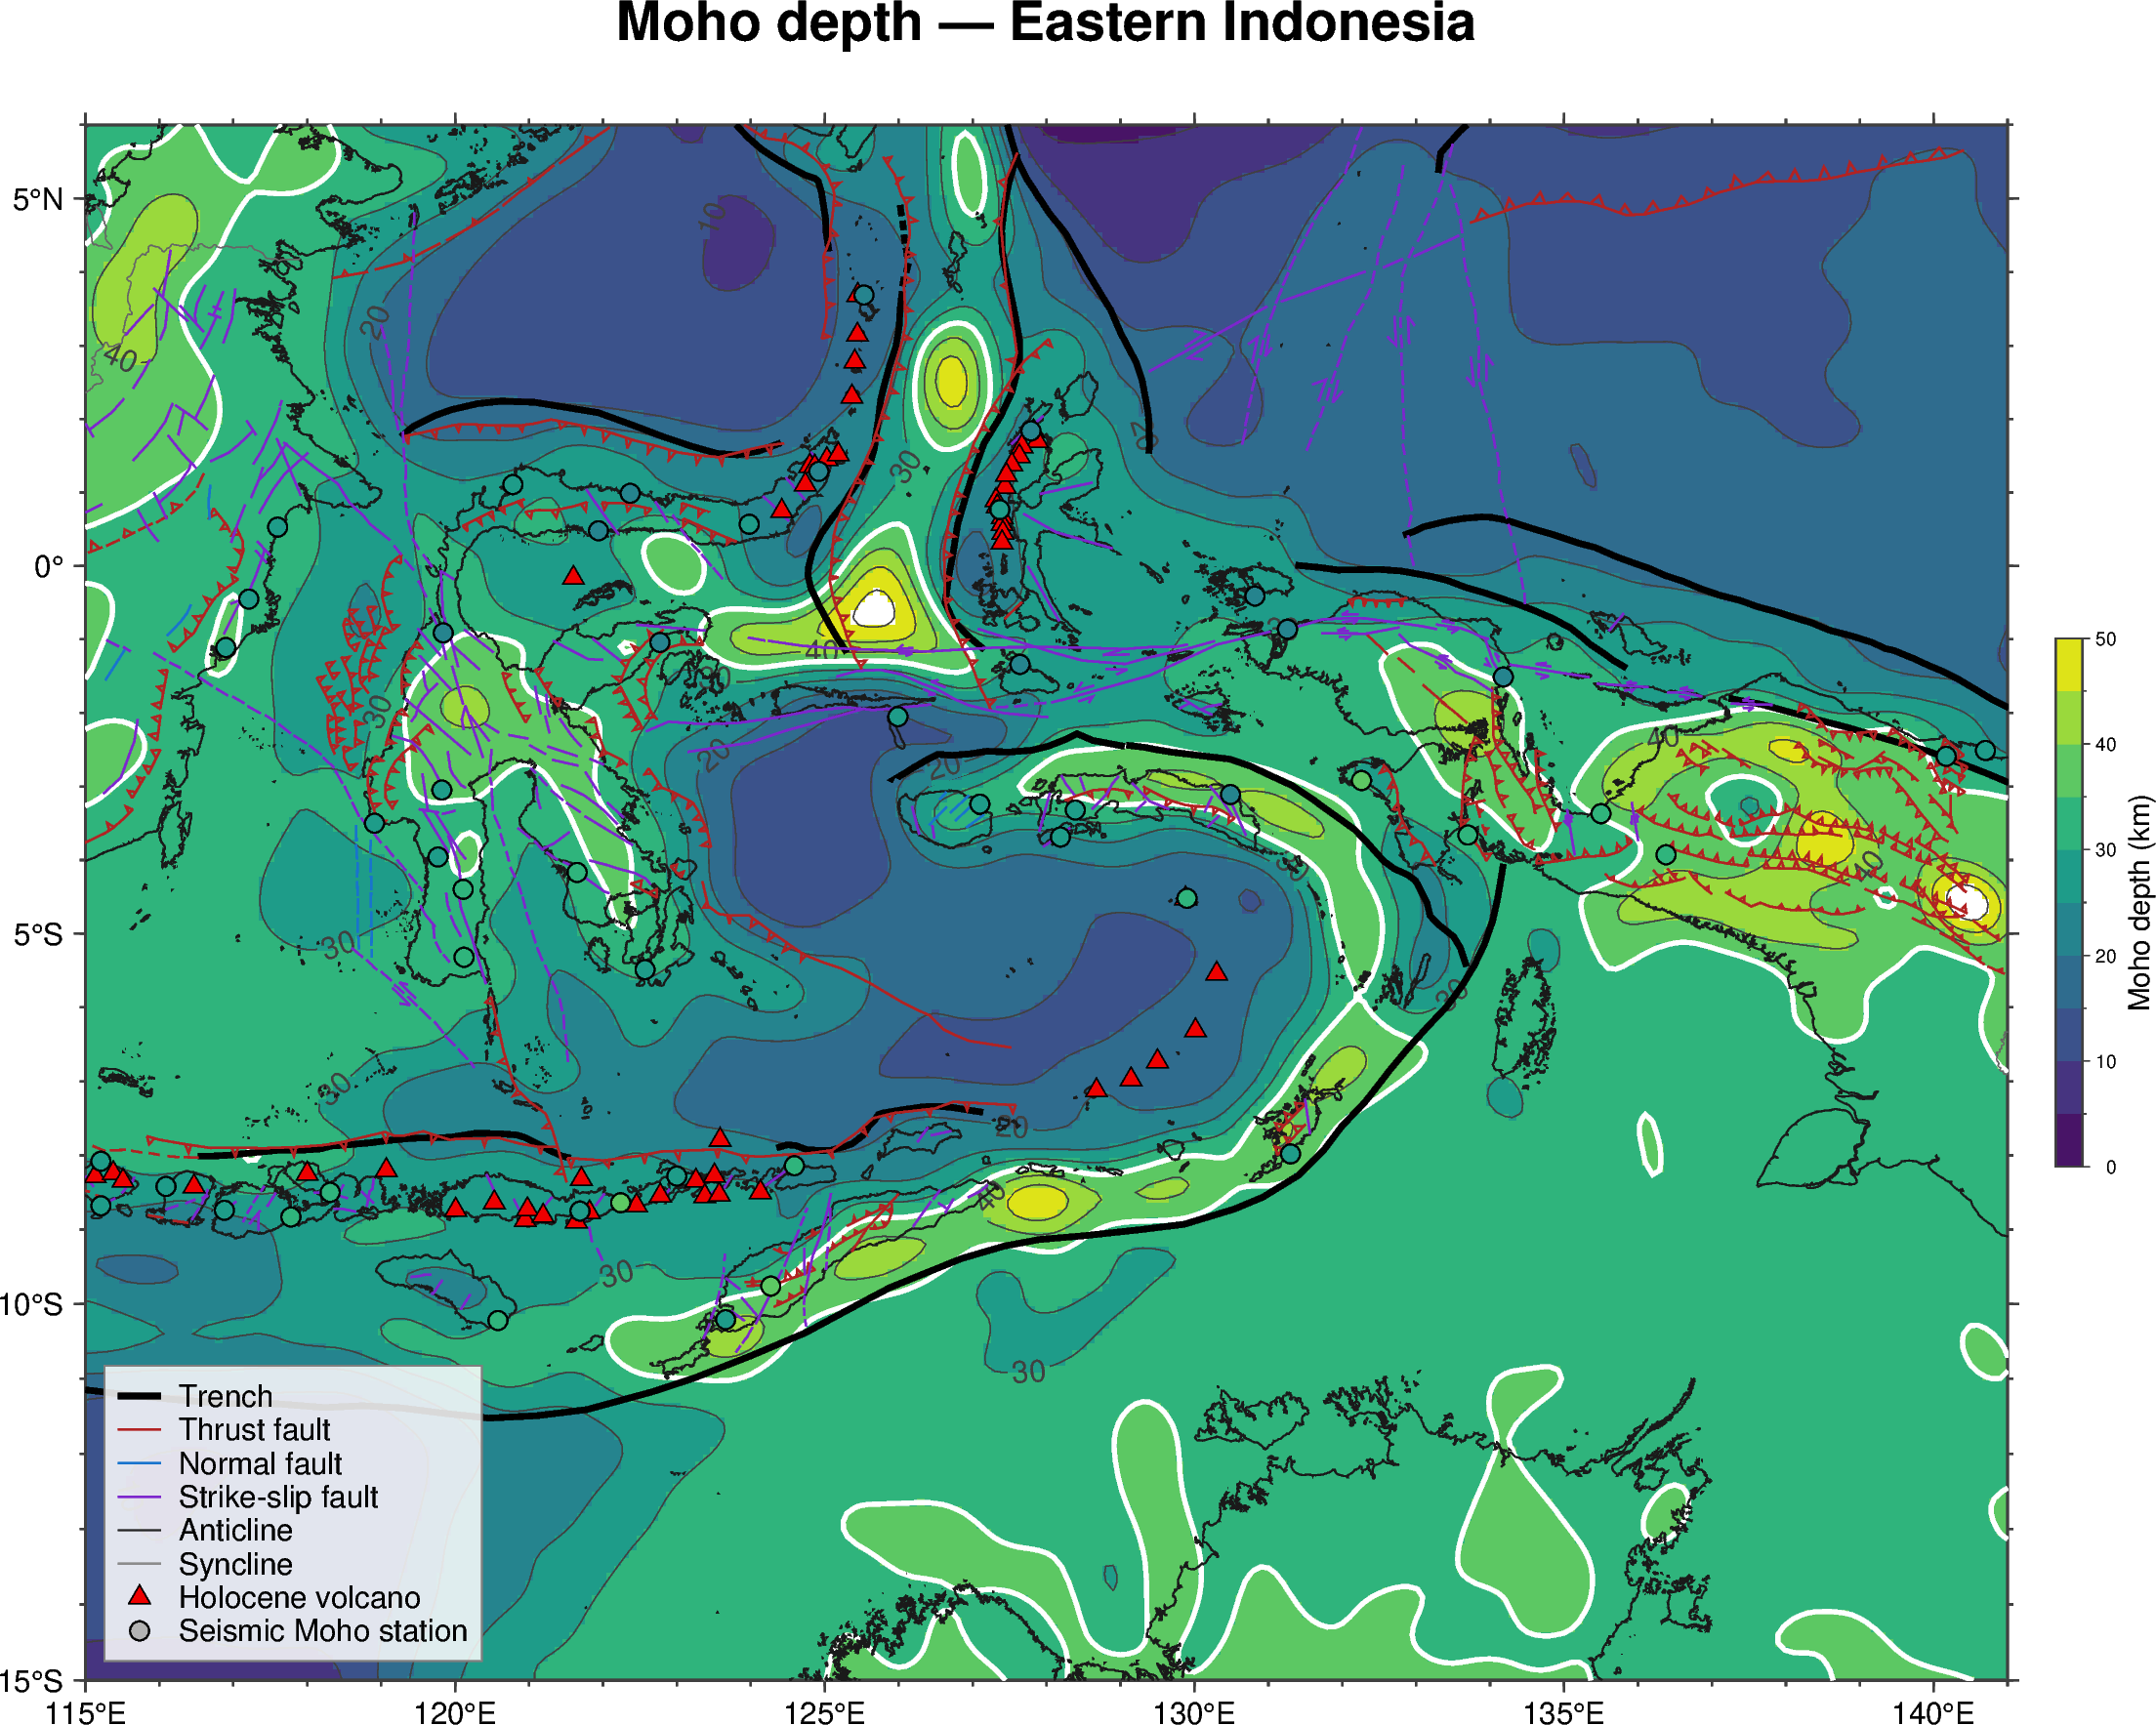
\includegraphics[width=\textwidth]{moho_east.png}
\caption{Eastern Indonesia (as Fig.~\ref{fig:west}): the Sulawesi--Banda--Papua
collision belt and the northern-Australia {AusMoho} overlap zone.}
\label{fig:east}
\end{figure*}

\label{lastpage}
\end{document}
